\documentclass[10pt]{article}
\usepackage[letterpaper]{geometry}
\geometry{verbose,tmargin=1in,bmargin=1in,lmargin=1in,rmargin=1in}
\usepackage{setspace}
\usepackage{ragged2e}
\usepackage{color}
\usepackage{titlesec}
\usepackage{graphicx}
\usepackage{float}
\usepackage{mathtools}
\usepackage{amsmath}
\usepackage[font=small,labelfont=bf,labelsep=period]{caption}
\usepackage[english]{babel}
\usepackage{indentfirst}
\usepackage{array}
\usepackage{makecell}
\usepackage[usenames,dvipsnames]{xcolor}
\usepackage{multirow}
\usepackage{tabularx}
\usepackage{arydshln}
\usepackage{caption}
\usepackage{subcaption}
\usepackage{xfrac}
\usepackage{etoolbox}
\usepackage{cite}
\usepackage{url}
\usepackage{dcolumn}
\usepackage{hyperref}
\usepackage{courier}
\usepackage{esvect}
\usepackage{commath}
\usepackage{verbatim} % for block comments
\usepackage{enumitem}
\usepackage{hyperref} % for clickable table of contents
\usepackage{braket}
\usepackage{titlesec}
\usepackage{booktabs}
\usepackage{gensymb}
\usepackage{listings}
\usepackage{cancel}
\usepackage[mathscr]{euscript}
\lstset{
    frame=single,
    	basicstyle=\ttfamily\small,
    breaklines=true,
    postbreak=\raisebox{0ex}[0ex][0ex]{\ensuremath{\color{red}\hookrightarrow\space}}
}

% for circled numbers
\usepackage{tikz}
\newcommand*\circled[1]{\tikz[baseline=(char.base)]{
            \node[shape=circle,draw,inner sep=2pt] (char) {#1};}}

\newcommand{\beq}{\begin{equation}}
\newcommand{\eeq}{\end{equation}}
\newcommand{\beqa}{\begin{equation}\begin{aligned}}
\newcommand{\eeqa}{\end{aligned}\end{equation}}

\titleclass{\subsubsubsection}{straight}[\subsection]

% define new command for triple sub sections
\newcounter{subsubsubsection}[subsubsection]
\renewcommand\thesubsubsubsection{\thesubsubsection.\arabic{subsubsubsection}}
\renewcommand\theparagraph{\thesubsubsubsection.\arabic{paragraph}} % optional; useful if paragraphs are to be numbered

\titleformat{\subsubsubsection}
  {\normalfont\normalsize\bfseries}{\thesubsubsubsection}{1em}{}
\titlespacing*{\subsubsubsection}
{0pt}{3.25ex plus 1ex minus .2ex}{1.5ex plus .2ex}

\makeatletter
\renewcommand\paragraph{\@startsection{paragraph}{5}{\z@}%
  {3.25ex \@plus1ex \@minus.2ex}%
  {-1em}%
  {\normalfont\normalsize\bfseries}}
\renewcommand\subparagraph{\@startsection{subparagraph}{6}{\parindent}%
  {3.25ex \@plus1ex \@minus .2ex}%
  {-1em}%
  {\normalfont\normalsize\bfseries}}
\def\toclevel@subsubsubsection{4}
\def\toclevel@paragraph{5}
\def\toclevel@paragraph{6}
\def\l@subsubsubsection{\@dottedtocline{4}{7em}{4em}}
\def\l@paragraph{\@dottedtocline{5}{10em}{5em}}
\def\l@subparagraph{\@dottedtocline{6}{14em}{6em}}
\makeatother

\newcommand{\volume}{\mathop{\ooalign{\hfil$V$\hfil\cr\kern0.08em--\hfil\cr}}\nolimits}

\setcounter{secnumdepth}{4}
\setcounter{tocdepth}{4}
\begin{document}

\title{MATH 228b: HW4... g2, 3}
\author{April Novak}

\maketitle

\section{}

The continuity equation is used to model the density of cars:

\beq
\frac{\partial\rho}{\partial t}+\frac{\partial f(u, \rho)}{\partial x}=0
\eeq

where \(\rho\) is the density of cars and \(f(u)\) the flux of cars, which is a function of the car velocity \(u\) and density. A road is treated as a continuum, such that no individual cars are modeled. Integrating the above over \(x_{i-1/2}\leq x\leq x_{i+1/2}\), where a node-centered finite volume method is to be used, gives:

\beqa
\int_{x_{i-1/2}}^{x_{i+1/2}}\left(\frac{\partial\rho(x,t)}{\partial t}+\frac{\partial f(u, \rho)}{\partial x}\right)dx=&0\\
\frac{\partial}{\partial t}\int_{x_{i-1/2}}^{x_{i+1/2}}\rho(x,t) dx+\int_{x_{i-1/2}}^{x_{i+1/2}}\frac{\partial f(u, \rho)}{\partial x}dx=&0\\
\frac{\partial}{\partial t}\int_{x_{i-1/2}}^{x_{i+1/2}}\rho(x,t) dx+f(\rho(x_{i+1/2}), u)-f(\rho(x_{i-1/2}), u)=&0\\
\eeqa

Then, integrating in time over \(t_{n}\leq t\leq t_{n+1}\) gives:

\beqa
\int_{t_n}^{t_{n+1}}\left(\frac{\partial}{\partial t}\int_{x_{i-1/2}}^{x_{i+1/2}}\rho(x,t) dx\right)dt+\int_{t_n}^{t_{n+1}}\left(f(\rho(x_{i+1/2}), u)-f(\rho(x_{i-1/2}), u)\right)dt=&0\\
\int_{x_{i-1/2}}^{x_{i+1/2}}\rho(x, t_{n+1}) dx-\int_{x_{i-1/2}}^{x_{i+1/2}}\rho(x, t_{n}) dx+\int_{t_n}^{t_{n+1}}\left(f(\rho(x_{i+1/2}), u)-f(\rho(x_{i-1/2}), u)\right)dt=&0\\
\eeqa

Multiplying through by \(1/\Delta x\), or the inverse of the mesh spacing:

\beqa
\label{eq:1}
\frac{1}{\Delta x}\int_{x_{i-1/2}}^{x_{i+1/2}}\rho(x, t_{n+1}) dx-\frac{1}{\Delta x}\int_{x_{i-1/2}}^{x_{i+1/2}}\rho(x, t_{n}) dx+\frac{1}{\Delta x}\int_{t_n}^{t_{n+1}}\left(f(\rho(x_{i+1/2}), u)-f(\rho(x_{i-1/2}), u)\right)dt=&0\\
\eeqa

Then, we can define the solution cell \(i\) spatial average as \(P\):

\beq
P_i^{n}\equiv\frac{1}{\Delta x}\int_{x_{i-1/2}}^{x_{i+1/2}}\rho(x, t_{n}) dx
\eeq

Likewise, the numerical flux is defined as the flux cell \(i\) temporal average:

\beq
F_{i-1/2}^n\equiv\frac{1}{\Delta t}\int_{t_n}^{t_{n+1}}f(\rho(x_{i-1/2}),t)dt
\eeq

Inserting these into Eq. \eqref{eq:1} gives the fundamental structure of the finite volume method. At this point, the numerical flux can be defined by a large magnitude of different methods. Godunov's method, which is essentially equivalent to an upwinding method, and Roe's method, which consists of an arithmetic average plus a stabilizing correction term, will be investigated in this question.

\beqa
P_i^{n+1}-P_i^n+\frac{\Delta t}{\Delta x}\left(F_{i+1/2}-F_{i-1/2}\right)=&0\\
P_i^{n+1}=&P_i^n-\frac{\Delta t}{\Delta x}\left(F_{i+1/2}-F_{i-1/2}\right)\\
\eeqa

Godunov's method specifies the numerical flux according to the value of the solution that would be present at the original Riemann discontinuity location after \(\epsilon\) time has elapsed. For scalar conservation equations, this essentially reduces to upwinding. 

\beqa
F_{i+1/2}=&\begin{cases}\textrm{min}_{\rho_i\leq\rho\leq\rho_{i+1}}f(\rho) & \rho_i < \rho_{i+1}\\
\textrm{max}_{\rho_i\geq\rho\geq\rho_{i+1}}f(\rho) & \rho_i>\rho_{i+1}\\
\end{cases}\\
F_{i-1/2}=&\begin{cases}\textrm{min}_{\rho_{i-1}\leq\rho\leq\rho_{i}}f(\rho) & \rho_{i-1} < \rho_{i}\\
\textrm{max}_{\rho_{i-1}\geq\rho\geq\rho_{i}}f(\rho) & \rho_{i-1}>\rho_{i}\\
\end{cases}\\
\eeqa

Roe's method combines an arithmetic average of two neighboring fluxes based on cell-centered values with a stabilizing correction term, giving the following numerical fluxes:

\beqa
F_{i+1/2}=&\frac{1}{2}\left(f(\rho_i)+f(\rho_{i+1})\right)-\frac{1}{2}u_{max}\biggr\lvert\left(1-\frac{\rho_i+\rho_{i+1}}{\rho_{max}}\right)\biggr\rvert(\rho_{i+1}-\rho_{i})\\
F_{i-1/2}=&\frac{1}{2}\left(f(\rho_{i-1})+f(\rho_{i})\right)-\frac{1}{2}u_{max}\biggr\lvert\left(1-\frac{\rho_{i-1}+\rho_{i}}{\rho_{max}}\right)\biggr\rvert(\rho_{i}-\rho_{i-1})\\
\eeqa

These two models are both used to model a traffic light turning green at \(t=0\). The initial condition specifies \(\rho_{-1/2}\), and in order to allow the simulation to evolve appropriately, a domain from \(-5,5\) is used (this should be increased if a longer time duration is studied). The density cannot simply be held at \(\rho_L\) at the traffic light, since this would not allow a rarefaction wave to develop, and so the actual boundary condition applied at each time step is to set the density at the very first spatial node (at \(x=-5\), outside the range of interest) to \(\rho_L\). The simulation results for several time steps are shown below, including \(t=2\). 

\begin{figure}[H]
\centering
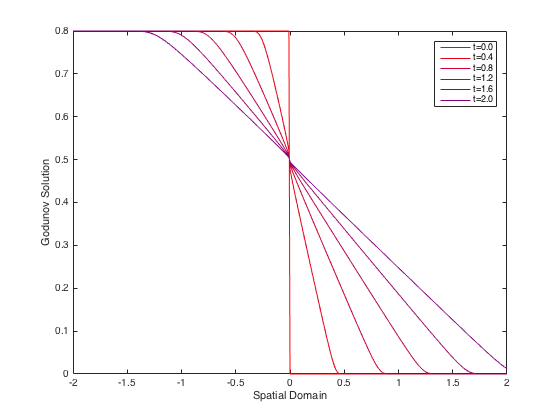
\includegraphics[width=0.6\textwidth]{figures/godunov1.png}
\caption{Solution at various time steps for the Godunov method.}
\end{figure}

\begin{figure}[H]
\centering
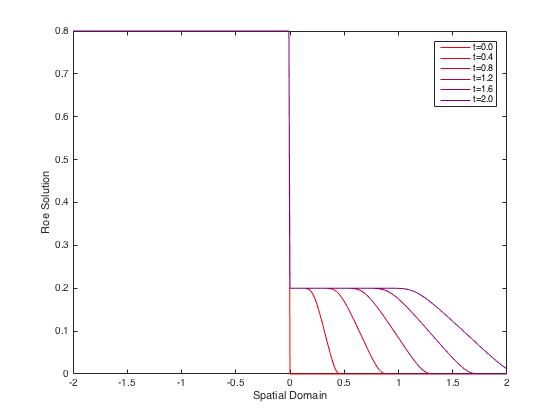
\includegraphics[width=0.6\textwidth]{figures/roe1.png}
\caption{Solution at various time steps for the Roe method.}
\end{figure}

By superimposing the two above graphs, it can be seen that at the front of the rarefaction wave, the Godunov and Roe solutions agree well with each other - they only give different results in the vicinity of the initial shock. For instance, by comparing the difference to either of the previous two plots, it can be seen that the difference drops to close to zero at around 1.25 for \(t=2\), even though the front of the rarefaction wave reaches out to about 2. So, both schemes capture the behavior far from the shock, but differ in the vicinity of the shock. In addition, there is a slight ``bump'' in the solution at the location of the traffic light for the Godunov solution, but by refining the mesh in both space and time, this small discontinuity disappeared, and is likely a remnant of the fact that the Godunov method (as well as the Roe method) is simply an approximation to the flux for each finite volume. 

The Godunov method gives the more realistic solution than Roe's method because Roe's method fails at resolving rarefaction waves, such as in this test problem. Roe's method is derived as a linearization about the averaged state \((\rho_i+\rho_{i+1})/2\) (for \(F_{i+1/2}\)). Due to this linearization, the solution will only consist of a single wave, as opposed to the \textit{two} waves that should normally travel from rarefaction waves. So, Roe's method entirely misses the left-going wave that causes the density to decrease to the left of the traffic light. For cases where the solution does not contain a rarefaction wave, Roe's method will perform well, since a shock consists of a single wave, moving either to the left or right. The code for this section is included in the Appendix.

\begin{figure}[H]
\centering
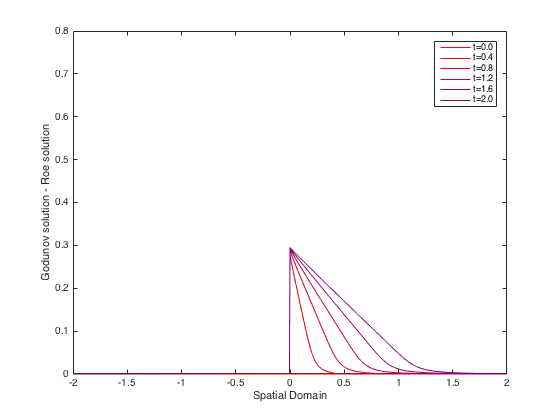
\includegraphics[width=0.6\textwidth]{figures/difference1.png}
\caption{Difference between the Godunov solution and the Roe solution at various time steps.}
\end{figure}





\section{}
Now, a traffic light is located at \(x_{i-1/2}\) for \(i=1\), i.e. the very first node has a traffic light at its left boundary. This traffic light will be simulated by setting \(F_{i-1/2}=0\) for the cell to the right of the traffic light, and \(F_{i+1/2}=0\) for the cell to the left of the traffic light. The figure below shows the solution at several time steps (over one full period) once reaching steady-state. Only results with the Godunov method are shown, since from Question 1, it was shown that Roe's method did not give good results for rarefaction waves. As can be seen from the figure below, the effects of the traffic light are correctly simulated - because the results at \(t=15.0\) exactly overlapped those at \(t=17.0\), results are shown at \(t=15.1\), just after the traffic light has turned red. A plateau of maximum density is reached, indicating that cars are arriving at the light and stopping still because they cannot drive forward. At \(t=16.0\), the light is just about to turn green, and a rarefaction wave develops after the light turns green as cars from behind the light can approach it, and cars beyond it continue to drive away. 

\begin{figure}[H]
\centering
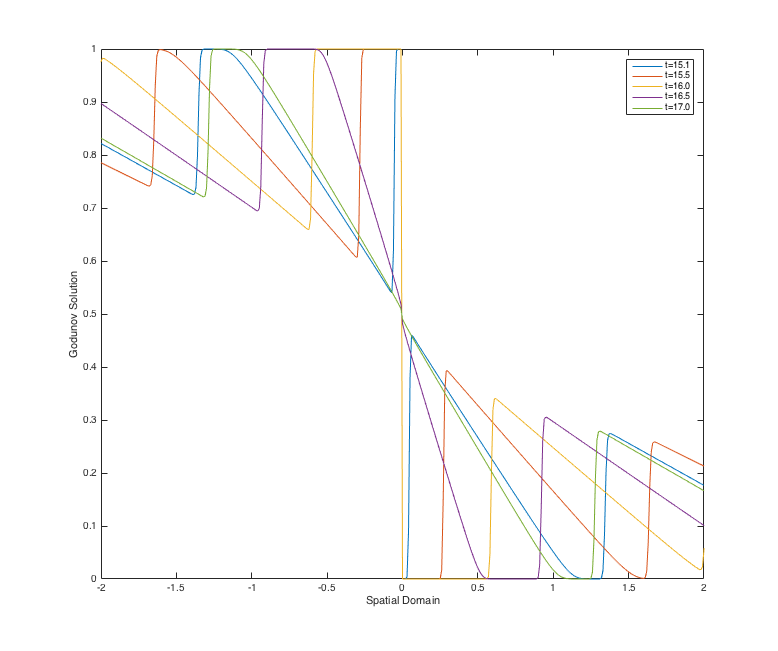
\includegraphics[width=0.75\textwidth]{figures/godunov2.png}
\caption{Godunov solution for a traffic light at \(x=-\Delta x/2\) with a period of \(2\), where the green light and red light each occupy half a period.}
\end{figure}

By conservation of the mass of cars per unit length of the road (i.e. continuity), the average flow \(\dot{q}\) can be computed at any point in the domain (and this is verified by computing the estimated flow at 50 different points in the domain). 

\beq
\dot{q}=\frac{1}{N_T}\sum_{n=1}^{N_T}f_n
\eeq

where \(N_T\) is the number of time steps per period, which for the time step given in Question 1 is 125. The average flow is computed to be roughly 0.251 cars/length\textsuperscript{2}time\textsuperscript{2}, where the units are consistent with those given in the problem. The code for this section is included in the Appendix.




\section{Appendix}
\subsection{Question 1}
\subsubsection{{\tt flux.m}}
This function calculates the flux given a density.
\lstinputlisting[language=Matlab]{flux.m}
\subsubsection{{\tt Godunov.m}}
This function calculates the left and right numerical fluxes using the Godunov method.
\lstinputlisting[language=Matlab]{Godunov.m}
\subsubsection{{\tt Roe.m}}
This function calculates the left and right numerical fluxes using the Roe method.
\lstinputlisting[language=Matlab]{Roe.m}
\subsubsection{{\tt Q1.m}}
This function calculates the solution for a single traffic light using both the Godunov and Roe methods.
\lstinputlisting[language=Matlab]{Q1.m}

\subsection{Question 2}
\subsubsection{{\tt Q2.m}}
This function calculates the solution for a cycling traffic light using Godunov's method.
\lstinputlisting[language=Matlab]{Q2.m}

\end{document}
